%\chapter{Background}
%%labels will help you to reference to certain images, tables, chapters, section, and so on...
%\label{background}


\chapter{Background and Related Work}
\label{relatedWork} 
\todo{check the label with the old and new texts after restructure}



%DELETEME: This chapter will cover all of your background information and related work. Background and related work are directly related to your thesis. Please do not place irrelevant content here which is a common mistake. Citing will be handled in the appendices.

\todo{redo}
In this chapter we discuss Amazon's state-of-the-art strategy
%before moving on to related work in other archetypes 
as it is important to introduce the implementation scope of voice assistants 
top down
%bottom-up 
prior to exploring the current context 
%within the same boundaries of voice assistants 
%then 
after comparing it to other approaches in the larger context of conversational bots as a whole from a technical and user experience point of view. 


%moved to gui section
%We start with a juxtaposition of Voice User Interface (VUI) to the Graphical User interface (GUI) respective to cognition and behavioural design which gets us to define new terminological foundation that will follow throughout this thesis.

%moved to chapter 3: to then elaborate on implementation requirements in Section \ref{frameworks_structs}. 


%DELETEME: Background represents underlying knowledge that is required to understand your work. The expected knowledge level of your readers can be set to the one of a bachelor or master student who just finished his studies (depending on what kind of thesis you are writing). This means that you do not need to describe how computers work, unless your thesis topic is about this. Everything that an avarage alumni from your field of studies should know does not need to be described. It turn, background information that is very complex and content-wise very near to you problem, can be placed in the main parts. Everyting else should be written here. Note: it is important to connect each presented topic to your thesis. E.g. if you present the ISO/OSI layer model you should also write that this is needed to understand the protocols you plan to develop in the main parts.







%#############################################################################
%###################### Related work  ########################################
%#############################################################################

%DELETEME: Related work respresents results from work that handled the same or a similar problem that you are addressing. This work might have used a different approach or might not have been that successful. Finding a paper / work that solved your problem in the same way you were planning to do is not good and you should contact your supervizor for solving this issue. Again, each paper / work has to be connected to your approach: other papers might have not chosen an optimal solution; they might not have been taking care of essential aspects; they might have chosen a different approach and you believe, yours will work better ...

%\chapter{Related Work}
%\label{relatedWork}

\todo{intro sentences}

\section{Digitilasation in the Public Sector}
\todo{bring up the Freiheit.org chart \cite{freiheit:digitalisierung}\\ 
	Talk about digitalisation in general (how there are talks in DE about autonomous driving and the related regulations - ref Haase)\\
	say that Germany cut in 2016 after UK, US, AT and even Bahrain short in e-government operations\\ bass}

\section{Worldwide Examples of Bots in E-Government}
\todo{
	
	\textbf{eingehen auf}\\
	- Wienbot\\
	- Singapore / LA / Ask Georgia...\\
	- LeiKa
	
	While we have no access to AskGeorgia from the German Amazon Store, we use the US store. %tab3an di f amrika fal mawdou3 mokhtalef, bas el fekra here is el design not the exact content
	\\
	witlingo: which builds voice-driven apps of all sorts for banks, universities, law firms, and others.\\
	aaron.ai\\
	
	say you chose wienbot and askgeorgia as german and english counterparts
	
}
\todo{
	For that we consider \textbf{the City of Vienna chatbot service \href{https://www.wien.gv.at/bot/}{``WienBot''}} given that it also uses German and the Alexa Skill \textbf{``\href{https://www.amazon.com/GeorgiaGov-Interactive-GTA-Ask/dp/B074XBQGTQ}{AskGeorgia}''} for a comparison in English.}

\todo{move / remove what is irrelevant
	In this section, we conduct a short survey of problems we can face with natural language
	\subsection*{topology of bots}
	\textbf{by platform:}
	-API.ai / 
	Facebook Messenger Chatbots /	
	-wit.ai /
	-motion.ai / Flask
	\textbf{by category}\\
	- leisure /
	- \href{https://www.forbes.com/sites/tomaslaurinavicius/2017/04/24/facebook-messenger-bots/\#4f61c16a66d8}{fun bots}  / 
	- productivity / 
	- more (graph from voicelabs report) \\
	- what are classic use cases for their use with prominent examples?\\ Booking tickets (e.g. airline bot)\\ %KLM
	- quick survey of respective 'AppStores'\\
	\textbf{by purpose}\\
	-physical locations (home, office, car, phone, in a business)\\
	Information bots\\
	\textcolor{magenta}{
		- mention available service types (information system as a "webpage/database")\\
		- vs an interactive bot that gives you customized information on demand
		hier soll der D115 Anwendungsfall "Beauskunftung" kurz erl\"autert werden\\
	}
	social bots\\
	\textcolor{magenta}{
		- with advantages / disadvantages\\
		- fake news / online reviews\\
	}
	more on AI in bots (optional)\\
	\textcolor{magenta}{
		- use of ML\\
		Handyversicherungsbeispiel\\
		- from business perspective, the bot is aiming to sell more polices,\\ 
		- the bot tries to determine if there is a nuance in the user's answer (machine acting as a judge!)
		- e.g. ``how did the phone fall off``
		- MKTG - Aufwand
	}
	IFTTT Applets for voice commands
}






\todo{ 2 \P \\
	
	\textbf{- Chatbot vs. human: }
	%what we used to do with facets vs a search mask predicting possible facets - we are at a stage where bots are like altavista..u tell alexa to open a skill like u tell altavista to look in pics or go to lexisnexis to do reserach. we are yet to reach the state of watson like google is to searches
	Analyze differences between bot and human response\\
	%human says long sentences and there is a fluid transition between dialog and monologue 
	-disadvantage: a bot wants a sentence broken down in small pieces to avoid errors in lengthy interpretation\\
	% otherwise, error margin too large.\\
	% this has to do with human language complexity.\\
	- \textbf{wrap-up:} can bots replace serivces offered by humans?
	-- mention transition from facets (Altavista) to metasearches to all-in-one (Google). \\
	-- chatbots as enablers in customer service industry\\
	-- conclusion: Although not impossible, it is a bit too far-fetched at this stage.\\
}

\todo{
	- structure of Hitlist on berlin.de  is provided by ITDZ -  as opposed to Versicherungsfirma z.B (ML tries to detect irregular patterns in case customer is lying).
	- unfortunately forums vs. FAQs did not work. if i want assistance, i want the customer to tell me the model number - and forums have mostly Schrott!\\
	what the bot curently achieved is at least not give wrong answers, sometimes says idk but it doesnt confuse u. same attitude like in lmny shops (nur unpassende antworten sind frustrierend!\\
}














%###################################################################################
%###################### Use Case in detail  ########################################
%###################################################################################
\section{Berlin as a Use Case}

%\subsection*{D115 and The Currently Deployed ``Virtual Bürgerassistent''}
\todo{
	- summarize infobroschuere\_ BMI08324\_screen\_barrierefrei.pdf\\
	-Use case im Detail\\
	-Welche Daten gibt es?\\	  
	-Was sind die Erwartungen?\\ 	
	- wie kann man die G\"ute des Systems beurteilen? \textbf{do not forget the surveyu made}\\   
	- Meist sollte man in diesem Kapitel die L\"osung schon im Auge haben, um die Erwartungen so zu formulieren, dass die L\"osung auch geeignet ist?\\ 
}



say that the bot is developed as a webapp using groovy

\todo{
	\textbf{current berlin.de bot}\\
	- dienstleistungen.json structure (finding the info through hierarchical nodes)\\
	- interpreting the nodes as intents\\
	- traversing the nodes (one level up then to next node)\\
	- no session/no persistence\\
	- explain how the json nodes map to intents and cores in solr etc
	
	%x	x	x
	%ooo ooo ooo
	%try first, go to second (kosten, zeit, rechtsgrundlage, ..) skip one if it has already been suggested.. hinweis..that is built into the xml
	%
	%the live service is different than the one at DAI
}

%%%%%%%%%%%%%%%%%%%%%

%\Tree [.Dienstleistungen.json created [.VP [.V is ] NP ] ]
%
%\Tree[.Dienstleistungen.json 	
%	[.NP [.Det \textit{the} ]
%		[.N\1 [.N \textit{package} ]]]
%	[.I\1 [.I \textsc{3sg.Pres} ]
%		[.VP [.V\1 [.V \textit{is} ]
%			 	   [.AP [.Deg \textit{really} ]
%				  		[.A\1 [.A \textit{simple} ]
%							  \qroof{\textit{to use}}.CP ]]]]]]]





\begin{figure}[h!]
	\caption{\mintinline{java}{Dienstleistungen.json}  - Primary Nodes}
	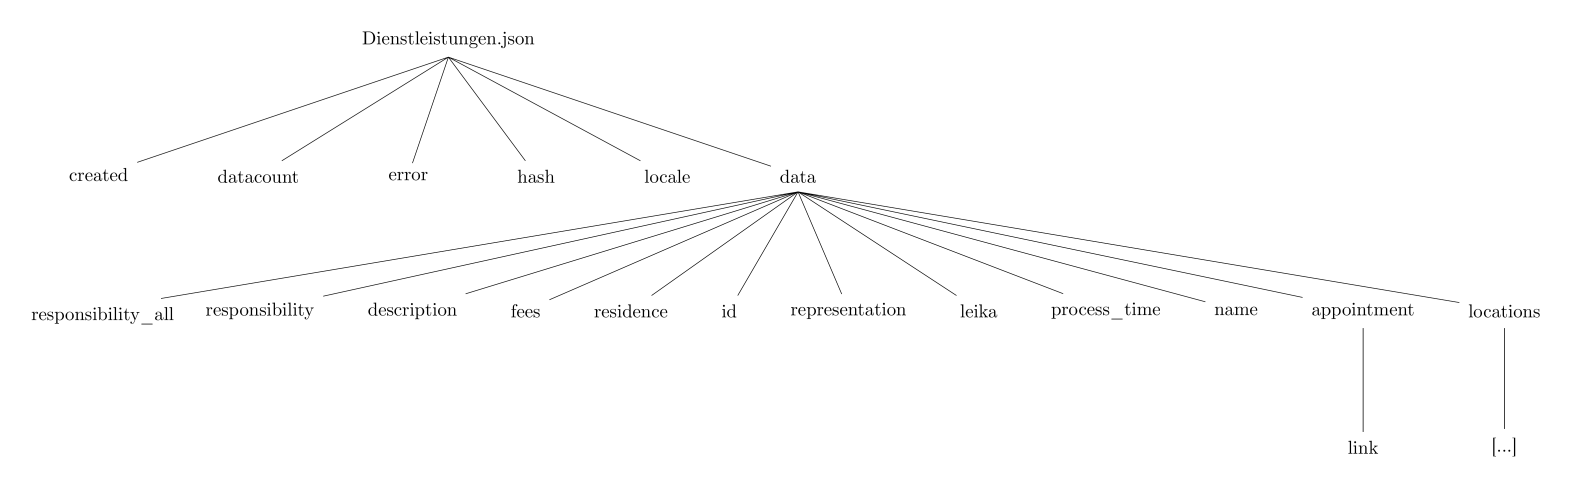
\includegraphics[width=\textwidth]{DLprim}
\end{figure}

\begin{figure}[h]
	\caption{\mintinline{java}{Dienstleistungen.json} - secondary Nodes}
	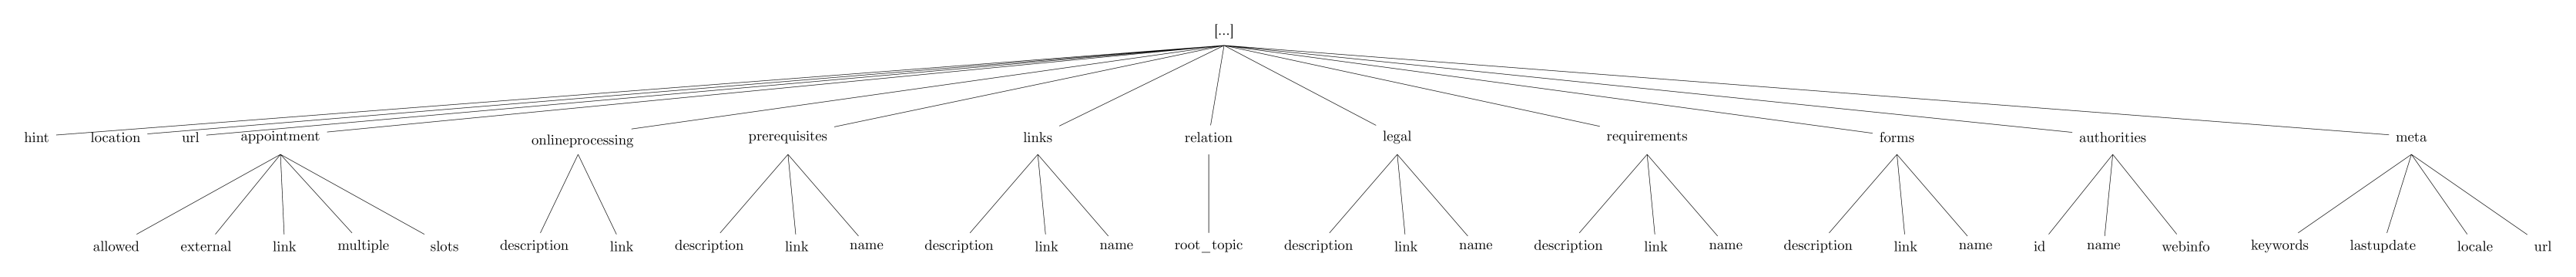
\includegraphics[width=\textwidth]{DLsec}
\end{figure}



provided in JSON for value lookup, the structure of the file is as follows: there are \inote{carry on - the structure}


started with 616 Intents in \lstinline|data| node (now 685 or so), each containing \inote{}
\todo{missing variables e.g. are required papers, flag: persönliche Vorsprache ja nein, ...}
\todo {change this into a table and add a tree list like the interaction model in appendix}

\begin{table}[htbp]
	\caption{relevant nodes in query results \mintinline{java}{Dienstleistungen.json} - Description}
	\label{dienstleistung:descr}
	\begin{tabu} to \linewidth {  r | l | l | l }
		key & type & ex. Value & description\\ \hline
		
		\mintinline{json}{id} & \mintinline{json}{int} & 326233 & public service ID on \href{https://service.berlin.de}{service.berlin.de} \\
		
		\mintinline{json}{d115URL} & URL \mintinline{json}{string} & ''https://service.berlin.de/dienstleistung/326233/'' & link to public service URL on  \href{https://service.berlin.de}{service.berlin.de} \\
		
		\mintinline{json}{d115Name} & \mintinline{json}{string} & Fiktionsbescheinigung & public service name as listed on \href{https://service.berlin.de}{service.berlin.de/dienstleistungen} \\		
		
		\mintinline{json}{ssdsAll} & \mintinline{json}{string} & ... & additional captive search terms, synonyms used by Virtueller Bürgerassistent. Found to be helpful in conversations with the chatbot \\		
		
		\mintinline{json}{d115Description} & \mintinline{json}{string} & ... & Introductory paragraph from the service web page. 
		Includes HTML tags \\ %like <\backslash br> and <ul ...> \\		
		
		
		%		
		%		\mintinline{json}{d115Synonym} & \mintinline{json}{string} & ... & captive search terms, synonyms created by Virtueller Bürgerassistent \\		
		%		
		%		\mintinline{json}{d115Position} & \mintinline{json}{string} & ... & captive search terms, synonyms used by Virtueller Bürgerassistent \\		
		%		
		%		\mintinline{json}{d115InfoLaw} & \mintinline{json}{string} & ... & Legal base for offering this public service \\		
		%		
		%		\mintinline{json}{ssdsAll} & \mintinline{json}{string} & ... & captive search terms, synonyms used by Virtueller Bürgerassistent \\		
		%		
		%		\mintinline{json}{ssdsAll} & \mintinline{json}{string} & ... & captive search terms, synonyms used by Virtueller Bürgerassistent \\		
		%		
		%		
		%		
		%		
		%		
		%		
		%		
		%		\mintinline{java}{string} & \mintinline{java}{responsibility}  & denoting in which city halls a service is available\\
		%		\mintinline{java}{boolean} & \mintinline{java}{responsibility_all} & a flag set to true in case the service is available in all local authority offices / service points\\
		%		
		%%	\mintinline{java}{HTML list string} & \mintinline{java}{ description} &  not unified and includes text \\
		%%%		\item  \lstinline|<string> not unified and might need to have an \lstinline|int| added to it and set to 0 in case service is free
		%		\mintinline{java}{int} & \mintinline{java}{residence} & \\
		%		\mintinline{java}{int} & \mintinline{java}{id} & \\
		%		x & \mintinline{java}{representation}  & x\\
		%		\mintinline{java}{long} & \mintinline{java}{leika}  & \\
		%		\mintinline{java}{string} & \mintinline{java}{process_time}  &  need to derive minimum, average and maximum service times instead of a string, as well as conditions\\
		%		\mintinline{java}{string} & \mintinline{java}{name} & the name of the service that would make sense to a human \\
		%		\mintinline{java}{node} & \mintinline{java}{appointment}  &  \\ 		
		%%		% then inner node 
		%%%		\begin{itemize}
		%%%			\item \lstinline|link| (Key value with URL to /terminveinbarung page) - check if orphan or if it is for each beh\"orde and in that case how it gets the right one
		%%%		\end{itemize}	 
		%		\mintinline{java}{node} & \mintinline{java}{locations}  & \\ 
		%%		% then inner node
		%%%
		%%			\mintinline{java}{hint}
		%			\mintinline{java}{int} & \mintinline{java}{sth} & location| one of the 12 authorities \\
		%%%			\item \lstinline|url| of that service at that authority
		%			\mintinline{java}{node} & \mintinline{java}{appointment} & (a second one)	 \\	
		%		\mintinline{java}{node} & \mintinline{java}{onlineprocessing}  & \\
		%		\mintinline{java}{node} & \mintinline{java}{prerequisites} & \\
		%		\mintinline{java}{node} & \mintinline{java}{links} & \\
		%		\mintinline{java}{node} & \mintinline{java}{relation}  & \\
		%		\mintinline{java}{node} & \mintinline{java}{legal}  & \\
		%		\mintinline{java}{node} & \mintinline{java}{requirements}  & \\
		%		\mintinline{java}{node} & \mintinline{java}{forms}  & \\
		%		\mintinline{java}{node} & \mintinline{java}{authorities}  & \\
		%		\mintinline{java}{node} & \mintinline{java}{meta}  & \\
	\end{tabu}
\end{table}














%#################################################################################
%###################### State of the Art  ########################################
%%#################################################################################
%\chapter{State of the Art}
%
%\sn{intro sentence}
%
%







%###################################################################################
%###################### Topic B             ########################################
%###################################################################################

%% moved to Chapter 3


































%###################################################################################
%###################### GUI/VUI ####################################
%###################################################################################

\chapter{The Voice as a User Interface} 
\label{vui}


We start with a juxtaposition of Voice User Interface (VUI) to the Graphical User interface (GUI) respective to cognition and behavioural design which gets us to define new terminological foundation that will follow throughout this thesis.

\section{GUI vs. VUI}
\label{guivsvui}

Visuals and Sounds can both communicate the same message even though they use a  completely different medium. One one hand, the premise that ``a picture is worth a thousand words'' can be valid based on the image but only assumes that we want to give a clear picture to the receiver. Communication through voice, on the other hand, can generally allow more room for interpretation. We think of an example where you would watch a football game on TV vs. the same game on radio, where listening to it allows each person in the audience group to imagine a different game for themselves, even though the match result are the same.


%%%Image

When we use written text, be it in a document or a street sign, or any label, we seek to mostly assure that all receivers understand the same message with a universal codification of what we want to express through the language we use. In this process, language becomes the common denominator for understanding and the short written text becomes purposefully designed to give in the best case a message not open to interpretation and so a foundation for an agreement or contract between the source and the destination of the message. It is a good medium of reference. 

%%%%%%%%%%%%%%%%%%%%%%%%%%%%%%%%%%%%%%%%%%
%voice message in airport - you can do your activity unobstructed
%%%%%%%%%%%%%%%%%%%%%
\section{Utility of Voice}
The utility of Voice comes handy with its different paradigm in numerous settings. 
For a passenger at the airport or an employee between meetings, 
%it is equally as helpful f
%as it would be for a  rushing to a meeting.
it can be more effective to ask questions through conversation than transform them into a query then type them on a screen,
%someone about the information you need quickly if you can ask it in a precise sentence quicker than you would write it, 
or visually navigate on a web page / mobile application until we reach the information we want. 
Today, this goes further beyond the simple use-cases to become an integral part of our fast-paced life, where we see companies like Ecobee getting around 40 percent of their sales through voice-based AI \cite{mit:Alexa} since their embrace about two years ago. The 10-year-old company's CEO elaborates that their customer “[...] have to fight traffic to get home, and then they have to feed the kids, diaper the baby, and who knows what else. [Ecobee] give them a hands-free way of getting something done while they’re in the midst of other tasks.”


Also, in terms of accessibility, blindness could sometimes make voice the only possible way to navigate or be aware of one's surroundings, e.g. a blind person crossing a street depends on the sounds coming from cars and traffic lights.
In that sense, voice can allow people to do their activities free-handed and unobstructed by actively engaging into reading activity, for instance having to look on a screen.
As our ambitions in connectivity become more complex, we have become more dependent on our phones in the last decade.
This is where use of a Voice User Interface could have the advantage of liberate us from the constant usage of our smartphones and moving from one screen to another. 
However, it is noteworthy that the trade-off between information exchange visually and through audio comes at a price. While both have their own advantages and disadvantages, it is important to understand that the context in which the medium is used is an important factor.

Hence, we need to differentiate between GUI design and that of a VUI. Since  we come from a GUI background thanks to the World Wide Web standards with HTML and CSS, it might not be most intuitive to apply the same concepts on VUI design simply since we start from the mindset that the GUI dictates how to use the software and the user has to understand this interface and deal with it as is.




\todo{It's important to understand that we are at the beginnings of VUI design, but are making progress, e.g. VUIs - should become seamless in an approach like this: \href{https://techcrunch.com/2017/08/30/amazon-and-microsoft-agree-their-voice-assistants-will-talk-to-each-other/}{Amazon and Microsoft agree their voice assistants will talk (to each other)}\\
- additional plugins are in the making, giving individual touch of sound based on profile (Alexa Podcast on the way to BXL)\\
- \href{https://recast.ai/blog/art-of-bot-design/}{art of bot design}\\
- \href{https://chatbotsmagazine.com/19-best-practices-for-building-chatbots-3c46274501b2}{best practices}
}



\inote{is this okay here or should it go in an appendix?}
\sn{andreas doesn't like to have more work done in this part. maybe put some of it in conclusion or remove completely, but i know you won't lol}

\section{Why Can't AI understand us}

AI has made giants leaps in the last few years. Thanks to neural networks, bayesian approaches in classification, decision trees and many other theories, we are capable of performing rigorous analyses on datasets
Considering that speech is one of the most complex forms of such, there are still various challenges that do not have a single strategy to tackle.

\begin{quotation}
What makes voice-based AI so appealing to consumers is its promise to conform to us, to respond to the way we speak—and think—without requiring us to type on a keyboard or screen. That’s also what makes it so technically difficult to build. We aren’t at all orderly when we talk. Instead, we interrupt ourselves. We let thoughts dangle. We use words, nods, and grunts in odd ways, and we assume that we’re making sense even when we aren’t \cite{mit:Alexa}.
\end{quotation}

When speech meets AI, there are a lot of language ambiguities to deal with and multiple contexts to understand. Since this is a field by its own and not the scope of this thesis, we only go briefly over a few categorical examples:
\begin{itemize}
	\item \textbf{Sytanx}: homonyms such as ``I \textit{present} you a \textit{present}.'' or ``The \textit{fly} wants to \textit{fly}''
	%homophones, homograph
	
	\item \textbf{Sematics}: metaphors, sarcasm, puns such as ``it’s raining cats and dogs''
	
	\item \textbf{Underlying Sentiment}: such as ``oh yeah, sounds very exciting'' when it's not.
	
	\item \textbf{Dialects}: enunciation such as \textipa{[dI"vE|9pm9nt]} \textit{(British)} and \textipa{[d9v"|Apm9nt]} \textit{(Indian)}

\end{itemize}

%\end{itemize}
%
%\begin{table}[h]
%	\begin{tabularx}{\textwidth}{r l l}
%		Syntax & Homonyms & \shortstack[l]{``I \textbf{present} you a \textbf{present}.''\\ ``The \textbf{fly} wants to \textbf{fly}''}\\
%		Semantic & Metaphors
%	\end{tabularx}
%	
%\end{table}
%

%\todo{
%	- \textbf{Why can't robots understand us:} language ambiguities - the need to understand context\\ the facebook vid\\
%--Syntactical: Homonyme\\ %fly, fly,  presently I’ll present you a present - now, give, gift
%--Semantic:  Methaphors, %“it’s raining cats and dogs”
%sarcasm, %“oh yea, sounds very exciting”
%and puns\\
%--dialects: enunciations\\
%--underlying grammar\\ %“what makes you abcd just now, ELIZA
%--underlying sentiment\\

%-\textbf{NLP Progress:} How does it help in enriching the bot experience\\
%--neural networks: help understanding language patterns and get better over time\\
%--thought vectors: helps connect different words with related meaingns\\
%--- link: fortschritt, und systemgrenzen heutzutage (kurze Sätze etc)
%}

While Machine Learning enables us to decode phrases not in the classical way in the past by randomly guessing the whole expression, our speech datasets grow and require analysis in further breadth and depth to deliver a sustainable Natural Language Understanding (NLU) engine.
So far, in the past six years our primary approach has changed due to the little progress made with it. Instead of trying to understand exact meanings, we work from
``imperfect matches at the outset, followed by rapid fine-tuning of provisional guesses'' \cite{mit:Alexa}. The learning part is involved by reinterpreting missed expressions \cite{aws:lex_webinar}. 
On one hand, neural networks help us understand language patterns and better the more frequently we use them, but can fail in the case of homonyms. \cite{mit:AILang} Thought Vectors on the other hand complement them by controlling the connection of different words with their related meanings %, which helps with homonyms for instance.

Depending on the system, it is therefore a rule of thumb that most AI-powered personal assistants like Siri or Alexa are in their early learning phases. In order to be able to make use of them in the future, the painful immaturity part has to come in effect. This limits us for instance to using short sentences to lessen the probability of the system misunderstanding us. And so, naturally, what distinguishes a good system from a better one is how fast it learns.


%a person whos a bit deaf and cant hear us. it happens with ppl too ya3ni}
Interestingly, a side effect of this indeterministic technique is that the voice assistant inadvertently simulates a person, who can sometimes not hear us, asks us to repeat a sentence or explain it in a different way. Although this is the same idea that a good system should have minimal fault tolerance, it is unprecedented to tackle a computer system on the consumer level with the idea that we might very much hit or miss the action we want to perform. On the other hand, though premature, it is evidence that a human has much more authority to a machine-powered brain.


Yet, although it might seem at the beginning that moving between both paradigms is easy, the more detailed system design gets, the trickier it becomes to transform GUI elements into text. Particularly with long texts. We will go over this in more detail about voice design guidelines in Section \ref{designGuide}.

\section{VUI Semantics}

Having the visual or haptic interface disappear is therefore a game changer for as soon as the user does not have direct instructions on how to deal with it, they start to improvise, or rather move away from the idea that the interface constrains them to the illusion that they define that interface and can control it. For instance, the user knows that they have to press only on a certain area of the screen to activate a button and actively move the mouse to that part. 
%Parallel to this in GUI; 
In other words,
when a user sees a  `save' button on a dialogue box, they relate to it in their head that the functionality behind that button lies in committing and keeping a persistent copy of the current state of the parent file to that dialogue. The label `save' describes in a visually expressive fashion what the user can or cannot do within this \textit{dialogue state}.


%Imagine you have an intent resembling the label on th button for ``ok''. with a function linked to it to perform a commit action, ...''}
%  

In voice on the contrary, a user is uninhibited in what they can and cannot say and the system is supposed to understand the \textit{intention}%~\ref{intents} 
of the user with \textit{the formulation}%~\ref{utterances} 
they just used.

%For us to hold on to that sentence, 
In order to translate the aforementioned with less ambiguity, we need to define the lexis we use for voice design utilized in most common chatbot and voice assistants constructs. 
%Just like most common chatbot constructs, Alexa Skills Kit (ASK) 
We divide the building model into intents%~\ref{intents}
, utterances%~\ref{utterances}
 and slots %~\ref{slots}. 
The Fulfilment part is taken care of through a back-end endpoint containing the programming and business logic to the interface, which also validate the slots before sending it onwards, similar to what JavaScript checks would do on a website. %We make the following words clear:

%\sn{Andreas suggests hochstufen - clear split required?}
\section{Terminology}
Before we discuss our choice of platform in Section \ref{choiceOfPlatform}, we already unveiled in Chapter \ref{introduction} that Alexa will be the underlying system. Thus we cap the elementary definitions of voice assistants with distinct Alexa-specific concepts and give meaning to the following terms: 

	\subsection*{Intent}~\label{intents}
	As the intention the user pursues with a spoken sentence. This translates to the action being executed upon the user's command based on mapping his/her words to this action.
	
	\subsubsection*{Utterance}~\label{utterances}
	As the wording a user picks to express his intent. For instance, to set the volume on a TV to quieter, we could say ``turn it down a nudge'', ``It's too loud'' or ``lower the volume''. Although all three sentences have the same meaning, linguistically, they are fully unrelated and only context makes us understand them, e.g. we have to know that ``it'' refers to the TV set in close proximity.
	
	\subsubsection*{Slot}~\label{slots}
	As a variable fo a certain type we define in our programme that belongs to a category of items. For instance, when someone says they would like to order a \textit{large} coffee, they assume that there is the option to have a small coffee, too. And so large and small refer both to the size of the coffee. Programmatically, we define \mintinline{java}{large} and \mintinline{java}{small} to be of type \mintinline{java}{size} of the coffee. Similarly, if there is the option to order a tea and a Cappuccino, it would be only fair to define \mintinline{java}{cappuccino} and \mintinline{java}{tea} to be of type \mintinline{java}{beverage}. Consequently, \textbf{slots} can be defined to any part of the sentence, where a parameter (here beverage or size) can be grouped into \textbf{slot types}. 

%\end{itemize}

%avoid using since you won't get indents easily	
%	\begin{minipage}{\linewidth}

	This idea is to be handled with care, though, since technically in most languages we can define a subject, a predicate and an object. Here is an example in English:
	
	% \! for negative spaces in math should be avoided as they do not work consistently
	% check here: https://tex.stackexchange.com/questions/67912/large-negative-spaces
	\[
	\underbrace{I}_\text{subject} \cdot
	\underbrace{would \ like  \ to \ have}_\text{predicate} \cdot
	\underbrace{
		\overbrace{{a}}^\text{number of items} +		
		\overbrace{lar\!ge}_\text{size} +
		\overbrace{cof \mkern-3mu fee.}^\text{beverage}
	}_\text{object} 
	\]
	
	When we design a voice system from scratch, we might have to make it understand how each of these sentence elements can be interchanged with another one of the same slot type. However, since utterances build on they idea of slot types, we can make delegate the system to understand what is important from the sentence through slot types and what other interoperable words are not relevant. In this example, if we say:
	
% \! for negative spaces in math should be avoided as they do not work consistently
	\[
	\overbrace{My \ brother} \cdot
	\overbrace{wants \ to \ order} \cdot
	\overbrace{ a + tall + cof\mkern-3mu fee.}
	\]
	
%	\end{minipage}

	it is not important to they system to understand at this stage who is going to drink the coffee. It should be more concerned with the intent; making the coffee, e g. sending a signal or instruction to a coffee machine.
	 
	Ultimately, it is up to us to draw the line on where we want to define a variable slot, that is relevant to the sentence being said by the user in context at a certain time in the conversation flow and where certain sentences would be as a whole giving the same intent
	
	
	\subsubsection*{Synonym}
	As a word that has the same meaning of another word that fills a slot. For instance, if we assume that a user says ``I want a \textbf{cup of jolt}'' they system should still be able to understand that they want a standard coffee. If, however, the user defines the type of coffee beans they want, such as `java' or `arabica', the system should still be able to differentiate between these and not consider them both as the plain `standard coffee', fulfilling a different intent. 
	
	\subsubsection*{Dialogue State}
	
	\subsubsection*{Dialogue Directives}
	
	\subsubsection*{Entity Resolution}	
	
	\subsubsection*{Fulfilment}
	
	\subsubsection*{Over-answering}

	\subsubsection*{Persistence}

%%%%%%%%%%%%%%%%%%%%%%%%%%%%%%%%%%%%%%%%%%%%%%%%%%%%%%%%%%%%%%%%%%%%%%%%
%\todo{
%	- how do you think of designing voice when you have a mobile mindset\\
%	- how do you think about screens when you have a mobile mindset and thinking about voice
%	subtle differnce
%	
%	- etkallem 3an el paradigm shift eli 7asal ma3 el mouse from cli if not already mentioned\\
%	- then 3an el smartphones and the web from wap etc (deskop version, responsive design, two versions, em instead of pt, relative, starting with a tablet and a phone then anything relative to those then when the standards showed that there won't be an only 15 inch and a 12 inch there will be everything in between, we changed the idea to include continuous units in the spectrum and not only discrete units)
%\cite{alexa_19} \\
%	- different screens, different mobile experiences and what does it mean
%}
%%%%%%%%%%%%%%%%%%%%%%%%%%%%%%%%%%%%%%%%%%%%%%%%%%%%%%%%%%%%%%%%%%%%%%%%










\chapter{State of the Art}
\label{stateofzart}




\todo{intro sentence}





%\sn{muss evtl weg}
\section{Analogies to the Introduction of Web 2.0}

\todo{web 2.0 was a weird word we didnt use and it became a hype then suddenly it disappeared after it has been defined.\\
it started with RSS and HTML stardards upgrade and now it's totally obvious where it goes.\\
no one uses RSS, but facebook and the idea of a feed would have not been born have we not started with RSS\\
}
With these introductory definitions we try to lay out a foundation for a standard, which is still in an experimental phase. Much like when tablets and smartphones were introduced to the market, the languages and framework used to render GUIs for the users had to adapt, e.g. with HTML5 and CSS3. In that transition, the experimental phase can be considered when browsers had to render a different page depending on the client. It started with a certain few screen resolutions that can be fixed, to offering a desktop and a mobile version and finally to the spreading of responsive design, the MPEG4 H.264 codec for video and so forth. When screen sizes and aspect ratios became also so diverse that it was hard to keep track of, website designers saw the importance of using different relative measuring units to present the website correctly (e.g. percentages for CSS classes, ems for fonts, etc.)


Since we mention context, in voice design we notice that the essence of an implementation lies in being able to think with a user mindset. In that respect, the developer of a voice design automatically becomes a designer to some extent. Part of that process is to understand where and when is the user going to request a certain intent. This helps us figure out how to offer the best user experience. For instance, it can be sometimes more effective to integrate the GUI inside the VUI, where the user gets to see relevant images, text or other elements related to the spoken responses by the visual assistant.\\


\todo{just a carriage return or add title? want to introduce here interaction model, dialog state, persistence, ...}

% As we present our solution in the Alexa environment and %, we would like to 
After familiarising ourselves with definitions %terms
that apply specifically to the Alexa platform,
%This was a prerequisite 
we are now able to understand the script building the \textit{interaction model} with the user. %and 
This helps us understand the code templates provided throughout the development process %. and is 
represented in JSON format. 
More information on the interaction model is availabe on the \textsc{Alexa Skill Design Guide.} \footnote{ \url{https://developer.amazon.com/docs/custom-skills/create-the-interaction-model-for-your-skill.html} and\\
	\noindent
	\url{https://developer.amazon.com/docs/smapi/interaction-model-schema.html}}


We cover here an excerpt of basic elements that we will later see more or less in the same structure of the JSON file containing the interaction model:



\todo{close paragraph above\\
explain json (this and LeiKa's) zu Ende\\
mention Alexa Voice Service and Products\\}

\begin{table}[h]
\caption[Interaction Model Schema]{\href{https://developer.amazon.com/docs/smapi/interaction-model-schema.html}{Interaction Model Schema (Skill Management API)~\cite{alexaDesignGuide} }}\label{interactionModel}
	\begin{tabularx}{\textwidth}{|l | l l l | }
	Field	&	Type	&	Description		&	Required \\ \hline
\lstinline|languageModel| &	object	& Conversational primitives for the skill	& yes\\
\_\_\lstinline|invocationName| &	object	& Invocation name of the skill	& yes\\
\_\_\lstinline|intents| &	array	& Intents and their slots	& yes\\
\_\_\_\_\lstinline|slots| (Intent Slots) & array & List of slots within the intent	& no\\
\_\_\lstinline|types| &	array	& Custom slot types		& no\\
\_\_\lstinline|samples|	& array	 & Sample utterances for the intent	& no\\

dialog & & & \\
elicitationRequired & & & \\
elicitation & & & \\
type (slot type) & & & \\
name (slot name) & & & \\

prompts & & & \\
\_\_ id  & & & \\
\_\_\_\_variations  & & & \\
\_\_\_\_\_\_type  & & & \\
\_\_\_\_\_\_value  & & & \\ \hline
			
	\end{tabularx}			
\end{table}






\todo{should I introduce concepts like entity resolution here already?}














%
%
%
% here used to be state of the art start
%
%
%







%%%%%%%%%%%%%%%%%%%%%%%%%%%%%%%%%%%%%%%%%%%%%
\section{Choice of Platform} %comparison AWS vs. el ba2i
\label{choiceOfPlatform}

\todo{moved from intro(was too detailed for up there):\\
	like Siri, Bixby, etc. \inote{put bixby somewhere else and be more precise on what u did based on section choice of platform} 
	such as Microsoft Azure Bot Framework, Amazon Lex and API.ai,
}
\todo{
	here you can talk about alternatives like Microsoft, etc, compare \textbf{pricing scheme}, say why you chose alexa (for its popularity mainly and 3ashan Api.ai et3amal abl keda\\
	%-AWS Lambda is free for the first one million calls per month\\
	-need to manage any SSL certificates when using AWS Lambda (since the Alexa Skills Kit is a trusted trigger).\\
	\url{https://developer.amazon.com/blogs/post/Tx213D2XQIYH864/announcing-the-alexa-skills-kit-for-node-js} very imp\\
	w 3ashan it's a whole established ecosystem. ma3 el ta7afozat eno amazon has an obscure position to data and privacy vs. siri masalan.\\
	3ashan ma3 siri me7tag iOS knowledge\\
	
	w ba2a 7aga like Maintain context(sesions), Intent chaining (khodlak kam screenshot men Azure)\\
	
	- on top of that, alexa does this cool thing where it gives\\
	
}


\todo{
	
	from a user point of view:
	\url{https://www.technologyreview.com/s/608571/alexa-understand-me/}
	SUSTAINED CONVERSATION\\
	In studies, AI platforms by Google, Apple, Microsoft, and Amazon all show different strengths. Google Assistant is the best on wide-ranging search commands. Apple’s Siri and Microsoft’s Cortana have other talents. Alexa does particularly well with shopping commands.\\
	
	Darren austin: \url{https://venturebeat.com/2017/06/27/how-amazons-alexa-hooks-you/}
	Alexa’s broader success resides in its ability to alleviate the stresses of an overbooked life. It’s the companion that’s always ready to engage.\\
	
}


Before deciding to develop for Alexa, we consider several options and evaluate their advantages and suitability for our requirements.


\begin{table}
	\begin{tabularx}{\linewidth}{r | l l l}
		& Alexa / AWS & API.ai & Microsoft Azure \\ \hline
		price & First million calls free per month & free & free \\
	\end{tabularx}
\end{table}

With Alexa as our choice, we agree to acknowledge the following considerations:




\subsubsection*{Availability}
\url{https://developer.amazon.com/docs/custom-skills/develop-skills-in-multiple-languages.html}
We choose to offer our skill only in Germany because our Skill's functionality is specific only within this geographical region. For that we configure the Skill to handle English (US) and German.

\begin{quotation}
	
	\item The skill is available only in the German skill store, due to the selected country distribution.
	\item The skill can be used by customers in Germany who have set their devices to use German.
	\item The skill can be used by customers in Germany who have set their devices to use English (UK).
	\item The skill cannot be used by customers in Germany who have set their devices to use English (US) or any other language.
	\item The skill cannot be used by customers in any other country, regardless of the language they've selected for their devices.
	
\end{quotation}


%%%%%%%%%%%%%%%%%%%%%%%%%%%%%%%%%%%%%%%%%%%%%







\todo{	
	
	\textbf{Intent fulfilment}
	%	-  Alexa Skills Kit+ Amazon Voice Services\\
	- mention how ability to react to everything is centralized at alexa somewhere \textbf{i.e. talk about SKILLS}\\
	- ability to retain sessions (explain requests/responses - GET/POST)\\
	- fullfilling intents\\
	- nested handlers\\
	\\
	skill service: code - business logic - handles json requests
	skil interface: configuration (developer portal)
	\\
	- difference to Lex \& Polly : \href{https://stackoverflow.com/questions/42982159/differences-between-using-lex-and-alexa}{diff alexa lex} \\
	
	- Major prob: lex is not in german\\
	- \href{https://www.youtube.com/watch?v=QxgdPI1B7rg}{Alexa Documentation}
}



%%%%%%%






%%%%%%%%%%%%%%%%%%%% choice of platform is kinda lost to where it belongs
%%%%%so we move it here for now to make a small intervention between terminology before we move on to alexa in detail
%%%%%%%%%%%%%%%




\todo{remove much from above \\
start with "proceding with Alexa, we introduce the backbone that operates it ...}

\chapter{Amazon's Ecosystem}
\label{amznecosys}
% alexa from user and developer sicht


In this chapter we discuss Amazon's state-of-the-art strategy
%before moving on to related work in other archetypes 
as it is important to introduce the implementation scope of voice assistants 
top down
%bottom-up 
prior to exploring the current context 
%within the same boundaries of voice assistants 
%then 
after comparing it to other approaches in the larger context of conversational bots as a whole from a technical and user experience point of view. 


\section{Amazon Web Services (AWS) + Alexa}


Getting started with Alexa as a platform for the first time might seem a little overwhelming especially since each component of it is being  constantly restructured since its debut release in November 2014 and with Q4 2016 being the beginning of its major market penetration success \cite{gartnerpreds17}. % AWS is constantly working on the interface and the sdk 
As throughout the course of this thesis these major changes occurred, %including even logo changes of the AWS modules!
%do some kind of changelog later
 we will go over the workarounds and circumventions to retain a working version of the software we present, discuss

\subsection*{AWS}
Amazon Web Services is a Cloud Computing service provider with a complete set of services to help build and run web applications ``reliably and securely at a cost and scale'' according to one's independent needs \cite{aws_website}.
It comes with agile abilities to adjust to various solution at a flexible scheme with benefits like multiple server farms globally (operating under different legal contracts with respect to data security and user privacy), caching, NoSQL, DevOps and so forth.


\subsection*{Alexa}
Alexa is a cloud-based voice service assistant platform by Amazon powering millions of devices \inote{with \{number of requests\} {daily|monthly}} on its own-branded devices like the Echo, Echo Dot, Tap, FireTV as well as cross-platform through mobile apps available through  \href{https://itunes.apple.com/de/app/amazon-alexa/id944011620?l=en&mt=8}{Apple's AppStore for iOS} and  \href{https://play.google.com/store/apps/details?id=com.amazon.dee.app&hl=en}{Google Play Store for Android} devices. Unlike Apple's approach with Siri for instance \footnote{as know from its policy on  new software and hardware products like the case with the iPhone, the Mac, etc.}, where including support for third-party integration on iOS's Service Development Kit (SDK), Amazon decided with the launch of Alexa to include non-Amazon developers right from the start by introducing a multitude of (SDKs) around the platform as part of AWS, e.g. Alexa Skills Kit SDK discussed further below.

So far, though the separation of AWS and Alexa's environments is not linguistically intuitive with the company's name labelled on every service component \footnote{see Etymology in Annex \ref{etymology}}, \href{http://www.amazon.com}{Amazon.com, Inc.} offers an array of web services through AWS that summarize all building blocks necessary to operate Alexa as a software for end-users. Of course with the introduction of the aforementioned devices, it becomes intuitive to call these `Alexa devices' since their primary purpose is to operate as Alexa clients. We refer to Alexa here only as the service offered by Amazon to consumers. Consequently, although Alexa comes as a fully packaged service to end-users, we can reduce it to a compilation of many micro-services provided by AWS. As most of these are available separately in the form of Software as a Service (Saas), we conclude that AWS incorporates the following components required to make Alexa come together and becomes a consumer of its own web services platform. 

%\cleardoublepage

\section{AWS Modules as Alexa's Building Blocks }
\inote{make logos as minipage objects or set as table / problem with footnotes}
%\inote{in print, make sure the following list goes on a spread (odd then even page number) with the image at the end of it for clarity}

listed in sequential order of importance, Alexa's service modules include but are not limited to: 

\begin{enumerate}

	\item[\href{https://aws.amazon.com/lex/}{\textbf{Lex}} \footnote{\url{https://aws.amazon.com/lex}}] \textit{for conversational interfaces using Natural Language Understanding, Text-to-Speech and Speech-to-Text} \\
	``a service for building conversational interfaces into any application using voice and text''\cite{aws_website}.
	While Lex is the most important backbone to make Alexa possible and can be a main operator of another software package to create a whole new category of voice assistants and conversational bots independent from Alexa, Siri etc., development for Lex was not available in German at the time of this research. We therefore decide to use the Alexa Skills Kit, which ultimately takes advantage of Lex and the other components described below under the hood. Lex and Alexa use the same deep learning techniques for natural language processing with the workflow described with the example in Figure \ref{lex_interactionExample} below. More information on Lex and its difference to Alexa are discussed in Appendix \ref{lexAlexa}.
%	
%	\begin{restoretext}
%		\begin{flushright}
%
%			
\includegraphics[width=1cm,height=1.1cm]{awslogos/lexlogo}
%		\end{flushright}
%
%	\end{restoretext}

	
	
	\item[\href{https://aws.amazon.com/polly/}{\textbf{Polly}} \footnote{\url{https://aws.amazon.com/polly}}] \textit{for speech synthesis\\}
	another ``service turn[ing] text into lifelike speech, allowing [developers] to create applications that talk'' \cite{aws_website} wile harnessing the power of deep learning. It is more or less the mouthpiece of Alexa built on top of speech synthesis algorithms.
	
%	
%	\begin{restoretext}
%		\begin{flushright}
%		
\includegraphics[width=1.06cm,height=0.9cm]{awslogos/pollylogo}
%		\end{flushright}
%	\end{restoretext}
	
	
	\item[\href{https://aws.amazon.com/transcribe/}{\textbf{Transcribe}} \footnote{\url{https://aws.amazon.com/transcribe}}] \textit{for automatic speech recognition using Speech-to-Text}\\
	which ``makes it easy for developers to add speech-to-text capability to [...] applications'' \cite{aws_website}. With Transcribe we are able to get text out of the user's voice before passing it into a format Alexa's backend would understand.
	
%	
%	\begin{restoretext}
%\begin{flushright}
%	
\includegraphics[width=1.2cm,height=0.9cm]{awslogos/transcribelogo}
%\end{flushright}
%	\end{restoretext}
	
% \todo{don't mention I'm using lambda until design chapter 3}

	\item[\href{https://aws.amazon.com/lambda/}{\textbf{Lambda}} \footnote{\url{https://aws.amazon.com/lambda}}] \textit{for intent fulfilment}\\
	Although Lambda is a versatile ``service [built] for a variety of real-time serverless data processing systems'' \cite{aws_website}, it can be used as an integrated server instance to host back-end code for intent fulfilment. %\ref{intent_fulfilment}.

	
%	
%	\begin{restoretext}
%\begin{flushright}
%	
\includegraphics[width=0.8cm,height=0.9cm]{awslogos/lambdalogo}
%\end{flushright}
%	\end{restoretext}
%




\item[\href{https://aws.amazon.com/dynamodb/}{\textbf{DynamoDB}} \footnote{\url{https://aws.amazon.com/dynamodb}}] \textit{for persistence storage}\\
acting as a nosql database table ...Although Lambda is a versatile ``service [built] for a variety of real-time serverless data processing systems'' \cite{aws_website}, \inote{we use it / it can be used} as an integrated server instance to host our back-end code for intent fulfilment%\ref{intent_fulfilment}.
We might as well use just any other privately or cloud-based server solution to host our code and use it as an endpoint for our software, however choosing Lambda takes away the overhead of linking the front-end with the back-end of the program we develop (an Alexa Skill as we describe below). 



\item[\href{https://aws.amazon.com/s3/}{\textbf{S3}} \footnote{\url{https://aws.amazon.com/s3}}] \textit{for resource storage}\\
standing for simple storage service, ...Although Lambda is a versatile ``service [built] for a variety of real-time serverless data processing systems'' \cite{aws_website}, \inote{we use it / it can be used} as an integrated server instance to host our back-end code for intent fulfilment%\ref{intent_fulfilment}.
We might as well use just any other privately or cloud-based server solution to host our code and use it as an endpoint for our software, however choosing Lambda takes away the overhead of linking the front-end with the back-end of the program we develop (an Alexa Skill as we describe below). 


	\item[\href{https://aws.amazon.com/iam/}{\textbf{CloudWatch}} \footnote{\url{https://aws.amazon.com/cloudwatch}}]
	\textit{for event logging}\\
	CloudWatch acts like the console for an operating system. It monitors all low-level events happening within the AWS sphere. In combination with Lambda it comes as handy tool to log events resulting at runtime once a Lambda instance is called and its code being executed and is used for debugging.
	
	
%	\begin{restoretext}
%\begin{flushright}
%	
\includegraphics[width=1.26cm,height=0.9cm]{awslogos/cloudwatchlogo}
%\end{flushright}
%	\end{restoretext}


	\item[\href{https://aws.amazon.com/iam/}{\textbf{IAM}} \footnote{\url{https://aws.amazon.com/iam}}]
	\textit{for identity access management within AWS}\\
	Identity Access Management (IAM) is a secondary service module regulating in the Alexa context in combination with Lambda the routing rights between internal Amazon endpoints. It also ensures compliance policies are enforced within and between AWS modules, as well as between AWS modules and other external services.
%	
%	
%	\begin{restoretext}
%\begin{flushright}
%	
\includegraphics[width=1.36cm,height=0.85cm]{awslogos/cognitologo}
%\end{flushright}
%	\end{restoretext}


	\item[\href{https://aws.amazon.com/cognito/}{\textbf{Cognito}} \footnote{\url{https://aws.amazon.com/cognito}}]
	\textit{for identity access management beyond AWS}\\
	like the rest of AWS's platform, Cognito is a scalable service module to perform user authentication and can be used in combination with an external endpoint instead of Lambda.
	
%		\begin{restoretext}
%\begin{flushright}
%	
\includegraphics[width=0.76cm,height=0.9cm]{awslogos/cognitologo_old}
%\end{flushright}
%	\end{restoretext}
	
\end{enumerate}

%\newpage

\begin{figure}[h]
	\caption[Interaction Between AWS Modules (Coffee Bot)]{Interaction between AWS modules in the use case of a ``Coffee Bot'' based on Niranjan \cite{aws:lex_webinar} }\label{lex_interactionExample}
	\centering
	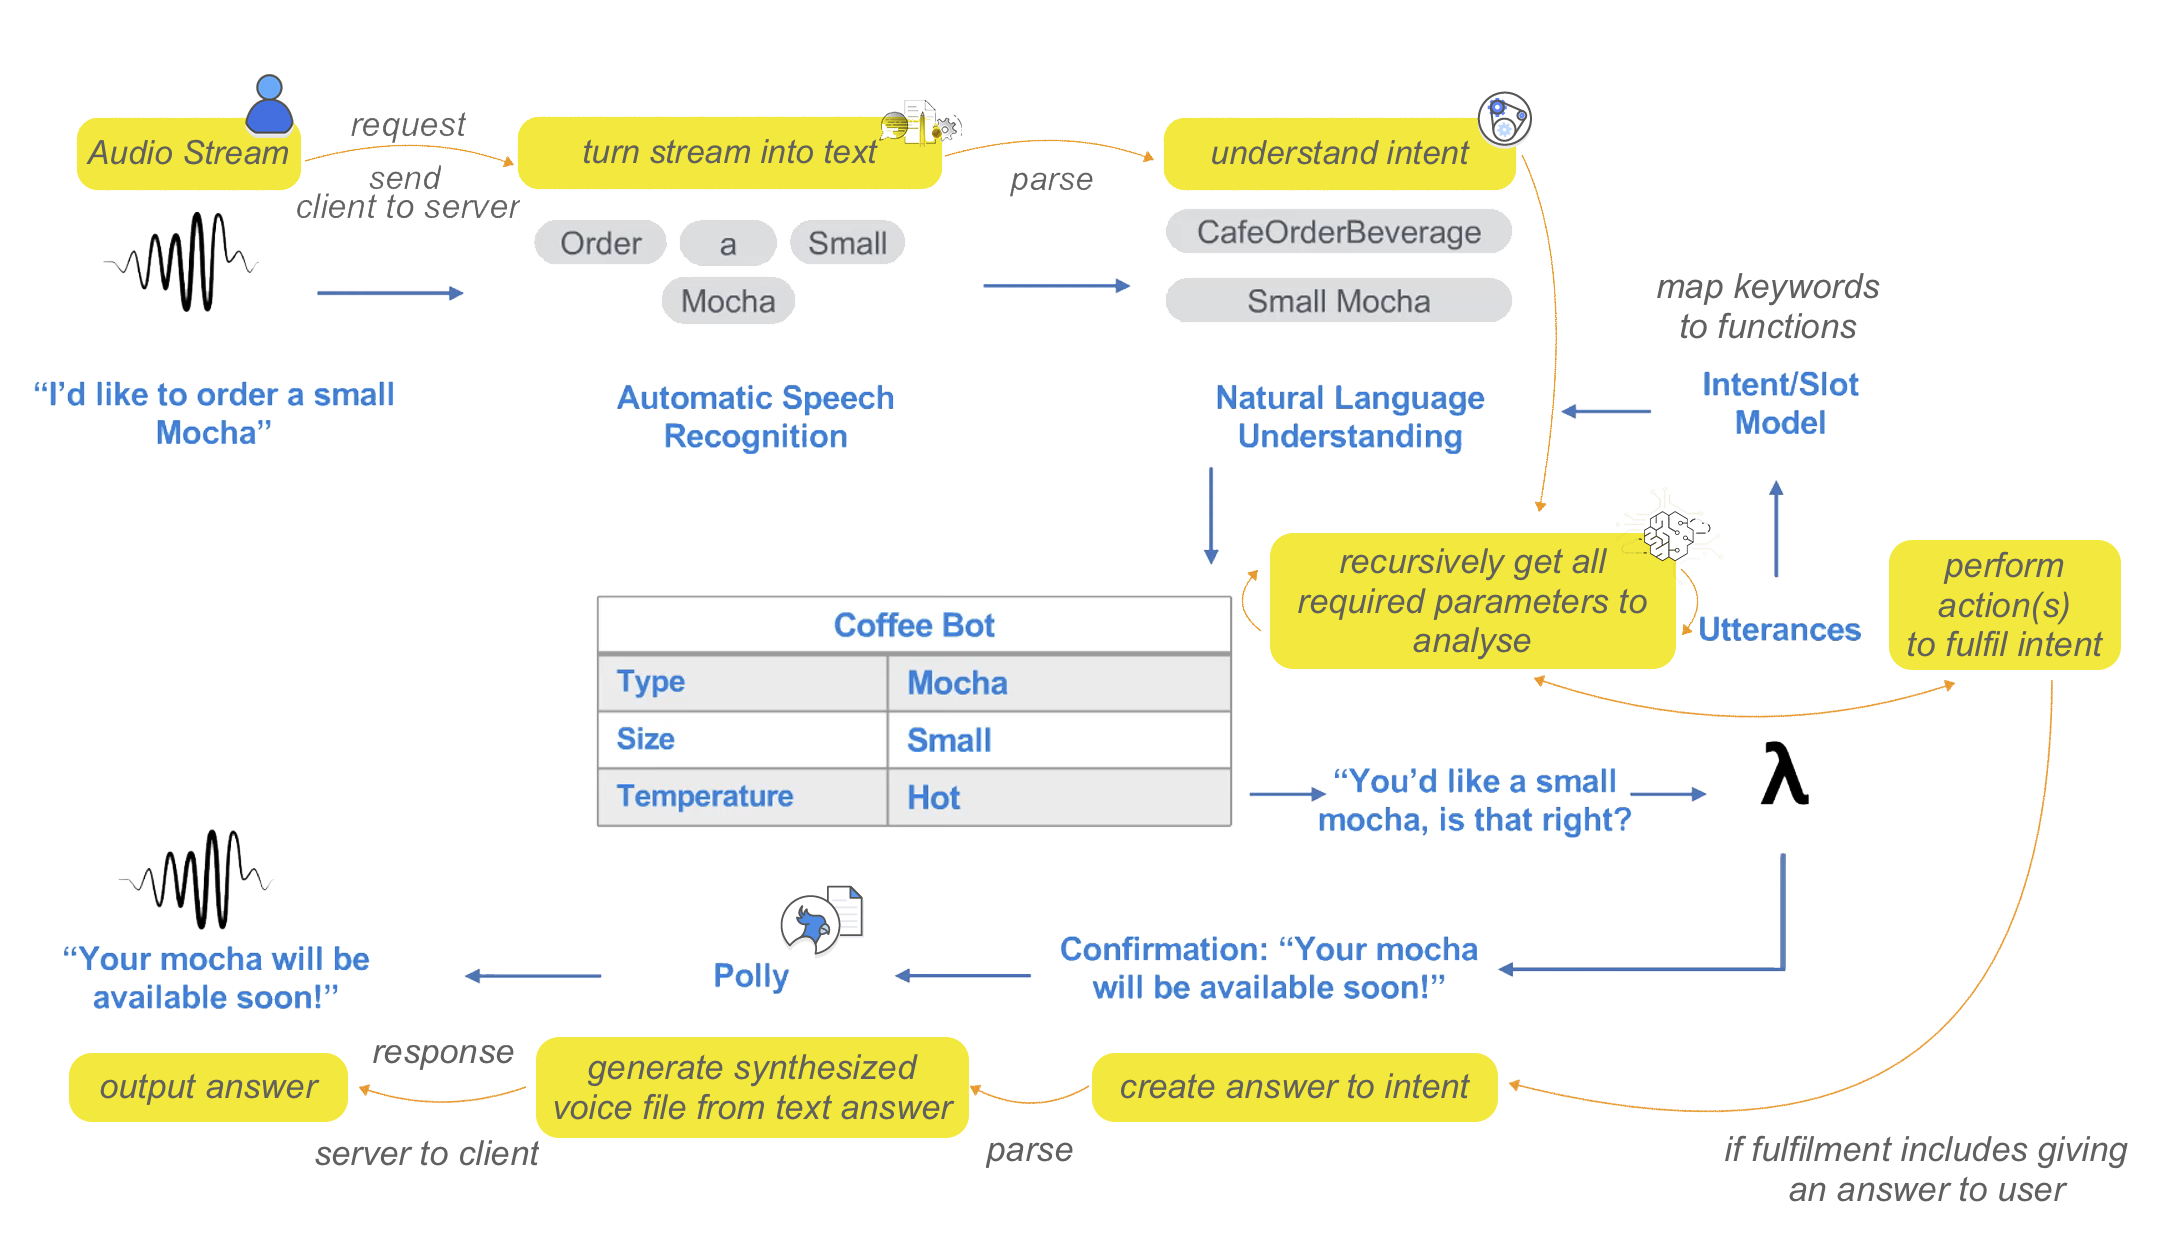
\includegraphics[width=14.8cm]{workflows/awstools.png}
\end{figure}
%
%\begin{wrapfigure}{l}{1.5cm}
%	\caption{Interaction between AWS modules in the use case of a ``Coffee Bot''}\label{lex_interactionExample}
%	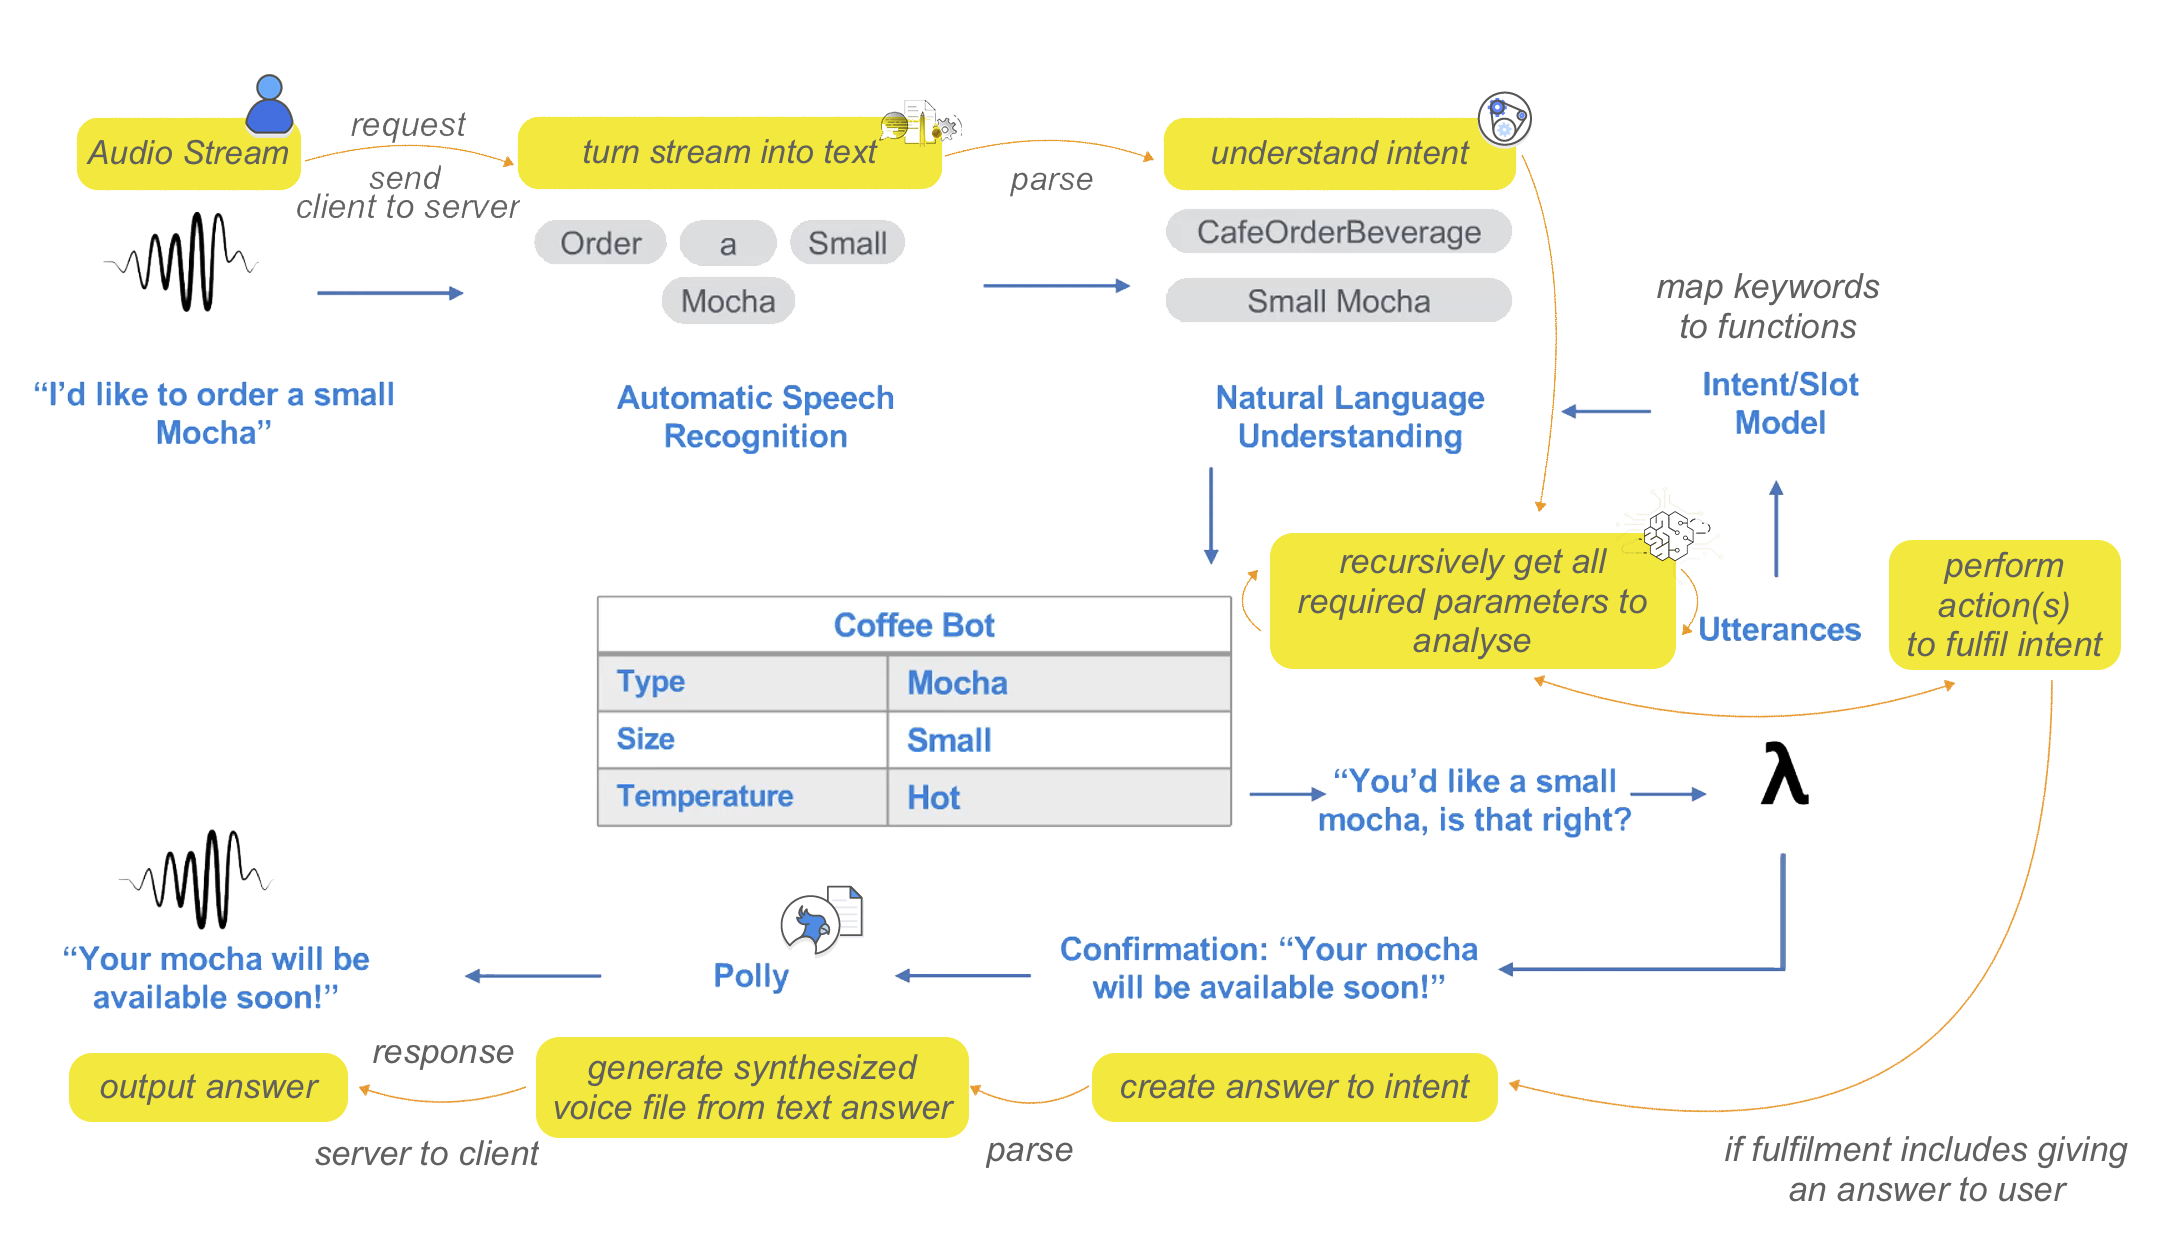
\includegraphics[width=10.5cm]{workflows/awstools.png}
%\end{wrapfigure}

putting different combinations of these and other building blocks interactively together generates the model for Alexa. In a world increasingly operated by Internet of Things (IoT), we describe a possible interaction in the example below for a use case of a hypothetical chatbot that operates a coffee machine using some of these service modules (Figure \ref{lex_interactionExample}).  Although this graphic describes how an end user would combine these modules to set up their own chatbot, this is the same workflow that Alexa uses. Hence, with Amazon's use of its own micro-services we infer that takes advantage of these to build a whole new ecosystem putting Alexa Skill developers as producers, end-users as consumers, and the Amazon website and Alexa App as a marketplace to mediate between the products (Skills) the developers produce to their target customers (end-users, country-specific or worldwide). From a marketing perspective Amazon achieves through Alexa a vertical diversification of its product programme (where existing AWS services result in a new product expanding the value chain) while simultaneously offering an extention of its aggregator-model marketplace model by playing as a mediator between the developers' role and that of end-users % (who of course could be developers, too)
% this is from what I concluded from MKT and GepIT lectures.. Prof. Küpper, Axel / Prof. Klasse-Talke, Kathrin




we can therefore describe the meta-model for Alexa similar as one %to that
of an application with several front-end and back-end components. Unlike in most GUI-based scenarios with an MVC design pattern \cite{wiki:mvc}, where the user uses the \lstinline|controller| to manipulate the \lstinline|model|, which in turn updates the \lstinline|view| appearing to the user, in a VUI scenario, we need to consider that the user's paradigm to the \lstinline|view| component is quite different. Before we dive into the VUI paradigm, we introduce Alexa's own implementation of it for third-party applications. These are broken down into the following elements for users and developers to comprise a holistic ecosystem:




\begin{itemize}
	\item[\textbf{Alexa Skills Kit}] although it is hard to define it as a complete SDK for Alexa and it is still in a continuous expansion phase, it is responsible for compiling the loosely coupled tools provided by AWS and others to act as an interface for the skill from a developer point of view. This fits into the rest of Amazon's scheme of focusing on interoperable micro-services that fit multiple purposes. It includes the following essentials:
	
	%Explain what the ASK SDK does
	
	\begin{itemize}
		\item [Alexa (Developer) Console] this is where all the developed skills live. It makes up a good representation of the JSON Files that include the language (interaction) models, the skill properties, the endpoints it uses and is where to submit the skill for publication
		\item[ASK CLI] \lstinline|ask-cli| A Command-Line Interface tool that interacts with the Alexa Console skipping the web browser. It is still in the making but has numerous functions to creating, deploying and testing our Skills. Download with Node Package Manager: \mintinline{bash}{npm install ask-cli}
		\item[Amazon Voice Service] \inote{products independent from Alexa, not sure if it's worth mentioning}
	\end{itemize}
	\item[\textbf{Alexa Skills Store}] where the end-user can preview the Skills before installing them, %know if they want it or not and by installing them, 
	Once installed, the own instance of Alexa becomes "smarter" by that Skill, which does not need to update from client side, since it is not hosted on the client (only sends requests to it). \footnote{This derives into a possible scenario where Alexa's AI becomes smarter then maybe in a few years the concept of Skills won't exist as a stand-alone anymore and would be integrated into Alexa's own brain without the user knowing and it would just be a hit or miss kind of thing.} for now the user does not need to think about updates since these happen in the back-end. 
	
	Continuous Skill Approval is the process of Amazon deciding whether each uploaded version / update is still fit for purpose, make the skill better or worse in conjunction with other skills on the Store % or change things to worse partly
\end{itemize}


\todo{remove clearpage before print}
\clearpage

\section{Alexa Interfaces}

Briefly going over the options available to use Alexa, we present and compare the different Hardware product lines and software solutions developed by Amazon or compatible with their voice assistant in terms of usability configurations, i.e. presentation of voice and graphical interfaces.

\subsubsection*{Hardware}
\begin{table}[htbp]
	\caption{Alexa Devices in Comparision}\label{alexaDeviceTable}
	\begin{tabularx}{\textwidth}{  r | l l l l  }
		
		category		& Speaker							& Tablet	& SmartHome	& TV	\\ \hline \hline \\
		curr. models	& \shortstack[l]{Tap, Echo \\ - Dot, - Plus}     & \shortstack[l]{Echo Show \\ Kindle Fire}    & Echo Spot & FireTV Stick \\ \hline \\
		screen  		& No      & 7.0" 		& 2.5'' round				&  HDMI Display      \\ \hline \\
		line out		& Yes      					        & \shortstack[l]{Show: Bluetooth \\ Kindle: Yes} & 	Yes & \shortstack{via HDMI \\ \textcolor{white}{text} }      \\ \hline \\
		Alexa on 	& Voice	Command					&
		\shortstack{ex. Fire HD 10\\Button Press}
		 %\shortstack[l]{K. 7, - HD 8:  btn press \\ - HD 10: voice cmd} 
		& Voice Command & %\shortstack{Button press \\ \textcolor{white}{text} }
		Button Press
	\end{tabularx}
\end{table}

% \inote{just make a comparison table, which one has a screen, which one has which capabilities with alexa}
%Echo, Echo Dot, Tap, FireTV


%then comes el software 
\subsubsection*{Software}

The Alexa app is not an Alexa interface yet (although this will change soon).

while the hardware models stated above are possibilities for testing, too, they do not primarily serve an optimal testing environment. There are better ways to automate Skill testing, for instance by running scripts that would send the transcribed text in the appropriate JSON format. This is helpful for conversations retaining sessions, so that one does not need to repeat the full conversation until one reaches the test breakpoint.

\begin{itemize}
	\item[EchoSim.io] ``an online community tool for developers that simulates the look and feel of an Amazon Echo'' \footnote{\url{https://echosim.io/}}
	\item[Alexa Simulator] an online simulator giving JSON responses and voice feedback to the requests sent. We interact with it either through voice or with JSON requests. Also available through the ASK CLI.
	\item[Reverb] An iPhone / Android app, allowing the interaction with the Alexa instance linked to an Amazon account. \footnote{\url{https:reverb.ai}} 
\end{itemize}



%%%%%%%%%%%%%%%%%%%%%%%%%%%%%%%%%%%%%%%%%%%%%%%%%%%%%%%%%%%%%%%%%%%%%%%%%%%%%





%###################################################################################
%###################### Topic C             ########################################
%###################################################################################











%Durchgestrichene bzw. lokalisierte/umbennante TODOs
%Done: Move node to implementation and don’t mention that you’re using lambda until In implementation chapter k
